\section{Pianificazione}

Con lo scopo di rispettare le scadenze descritte in questo documento è stata redatta la pianificazione del lavoro traendo ispirazione dalle attività previste nei processi di Fornitura e Sviluppo descritti nello standard ISO/IEC 12207:1995. Di conseguenza abbiamo suddiviso il lavoro nelle seguenti macro-fasi:
\begin{itemize}
	\item{\textbf{Attività preliminari di avvio ed analisi dei requisiti}};
	\item{\textbf{Progettazione architetturale}};
	\item{\textbf{Progettazione di dettaglio e codifica}};
	\item{\textbf{Validazione e collaudo.}}.
\end{itemize} 
In base alle scadenze inserite ad inizio documento, le macro-fasi saranno suddivise in questi periodi temporali:
\newline
\begin{table}[!htpb]
	\centering
	\renewcommand{\arraystretch}{2} 
	\rowcolors{2}{gray!25}{white}
	\begin{tabular}{|l|l|l|}
		\hline
		\rowcolor{orange!50}
		\textbf{Fase} & \textbf{inizio} & \textbf{fine}\\
		\hline
		Attività preliminari di avvio ed analisi dei requisiti & 15/11/2018 & 14/01/2019 \\
		\hline
		Progettazione architetturale & 22/01/2019 & 08/03/2019\\
		\hline
		Progettazione di dettaglio e codifica & 16/03/2019 & 12/04/2019\\
		\hline
		Validazione e collaudo & 20/04/2019 & 10/05/2019\\
		\hline
	\end{tabular}
	\caption{Pianificazione}
\end{table}
\newline Queste fasi vengono inserite in un diagramma di Gantt\pedice. dove le milestone\pedice sono assunte come principali scadenze di ogni fase. In questi diagrammi ogni attività è rappresentata tramite le sue sotto attività.
\newline Avendo in mente l'obiettivo di far ricoprire ad ogni membro del gruppo tutti i ruoli, ogni macro-fase è stata divisa in 2 parti così da avere un momento definito per il cambio di ruolo e per fare una verifica intermedia al periodo per valutare l'avanzamento del lavoro. 

\newpage
\subsection{Attività preliminari di avvio ed analisi dei requisiti}
Il periodo preliminare di analisi si svolge dal 15/11/2018 al 14/01/2019 e partono dalla formazione del gruppo terminando poi alla prima milestone ovvero la consegna dei documenti. \newline
Le attività principali sono le seguenti:
\begin{itemize}
	\item\textbf{Norme di progetto:} questo è il primo documento poiché contiene tutte le norme atte a regolare internamente il gruppo Dream Corp. che spaziano dall'indentatura del codice alle regole per stendere i documenti stessi;
	\item\textbf{Studio di fattibilità:} redatta dagli Analisti questa è un' attività bloccante per l'inizio dell'analisi dei requisiti. Consiste in un analisi dei pro e dei contro dei vari capitolati con il fine di una scelta ponderata del capitolato;
	\item\textbf{Analisi dei requisiti:} dopo aver scelto il capitolato è necessario approfondire i requisiti richiesti dalla proponente. Svolto ancora una volta dagli Analisti;
	\item\textbf{Piano di progetto:} questa attività è bloccante per la stesura della lettera di presentazione. Viene svolta dal Responsabile che ha lo scopo di analizzare le attività necessarie e la loro scadenza al fine di garantire la  buona riuscita del progetto mentre L'amministratore analizza i rischi nei quali il gruppo Dream Corp. può incombere durate il percorso. Inoltre in questa attività vengono stabilite le risorse disponibili per l'intero progetto;
	\item\textbf{Piano di qualifica:} in questa attività viene redatto il documento \textit{Piano di Qualifica} che ha lo scopo di individuare dei metodi per garantire la qualità del prodotto;
	\item\textbf{Glossario:} questa attività consiste nella redazione del \textit{Glossario}, dove verranno inseriti tutti i termini considerati possibilmente ambigui;
	\item\textbf{Lettera di presentazione:} attività che consiste nello studio autonomo di ogni membro del gruppo e, soprattutto, nella preparazione del materiale di supporto per la stesura della \textit{Lettera di presentazione} necessaria per il gruppo al fine di essere scelto come fornitore.
\end{itemize}

\begin{figure}[!htpb]
	\centering
	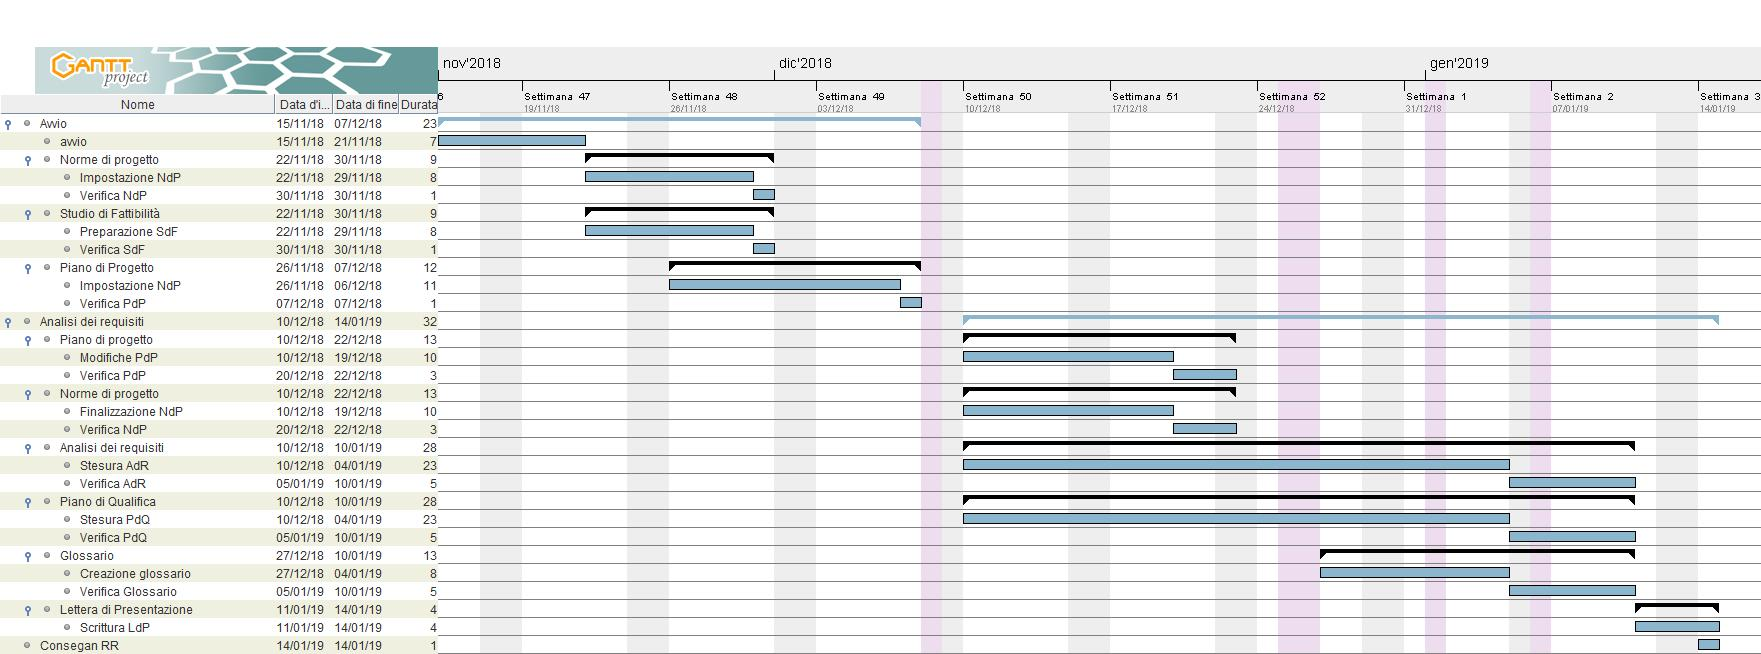
\includegraphics[width=\textwidth]{Gantt_prima_fase.jpg}
	\caption{Diagramma di Gantt del periodo di Analisi}
\end{figure}

\begin{figure}[!htpb]
\centering
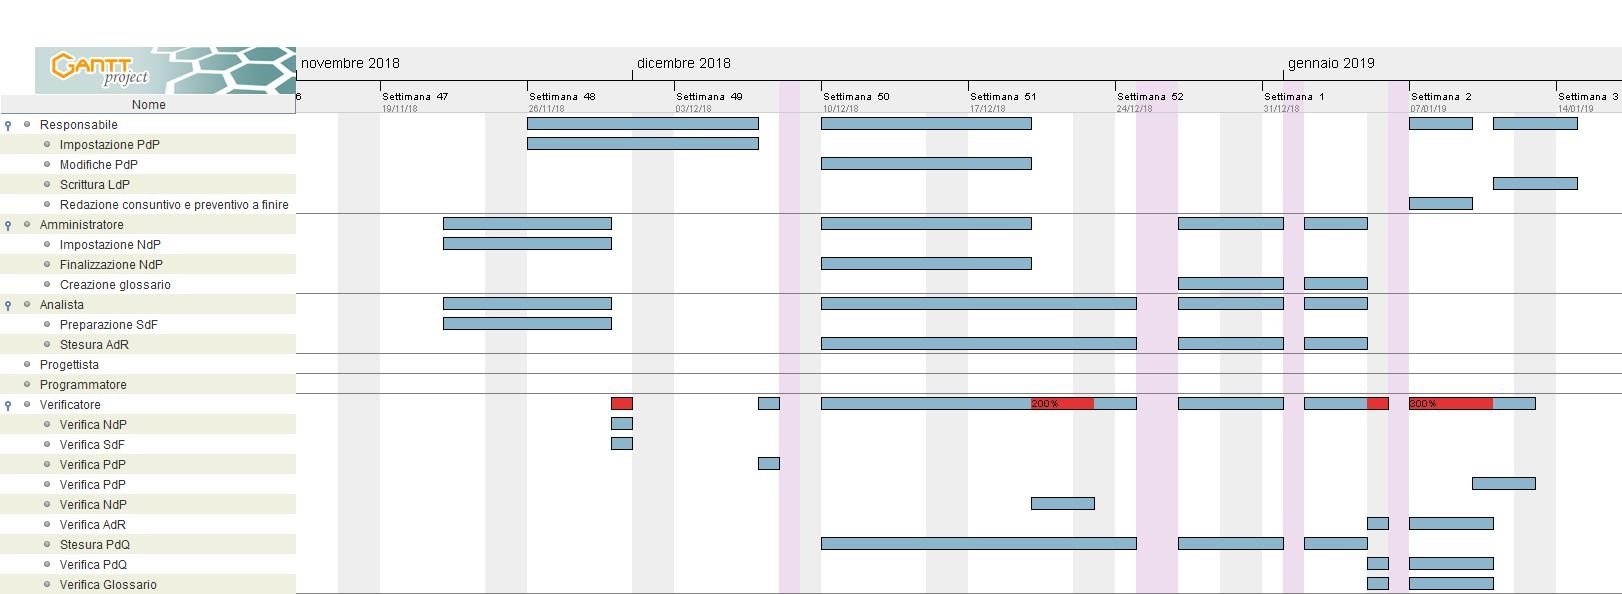
\includegraphics[width=\textwidth]{Gantt_prima_fase_risorse.jpg}
\caption{Diagramma di Gantt delle risorse del periodo di Analisi}
\end{figure}

\begin{table}[!htpb]
	\centering
	\renewcommand{\arraystretch}{2} 
	\rowcolors{2}{gray!25}{white}
	\begin{tabular}{|c|p{4.5cm}|p{4.5cm}|}
		\rowcolor{orange!50}
		\hline
		\multicolumn{3}{|c|}{\textbf{Suddivisione temporale}}\\
		\hline
		\textbf{Ruolo} & \textbf{15/11/18 - 10/12/18} & \textbf{11/12/18 - 14/01/19} \\
		\hline
		\textbf{Responsabile} & \daG & \pie \\
		\hline
		\textbf{Amministratore} &\parbox{4.5cm}{\gia \\ \mat} & \mar\\
		\hline
		\textbf{Analista} & \parbox{4.5cm}{\pie \\ \mic} & \parbox{4.5cm}{\daG \\ \daL \\ \mat} \\
		\hline
		\textbf{Progettista} & - & - \\
		\hline
		\textbf{Programmatore} & - & - \\
		\hline
		\textbf{Verificatore} & \parbox{4.5cm}{\daL \\ \mar} & \parbox{4.5cm}{\mic \\ \gia} \\
		\hline
	\end{tabular}
	\caption{Suddivisione temporale del periodo di Analisi}
\end{table}

\clearpage
\subsection{Progettazione Architetturale}
	\subsubsection{prospetto orario}

\begin{table}[h!]
	\centering
	\renewcommand{\arraystretch}{2} 
	\rowcolors{2}{gray!25}{white}
	\begin{tabular}{|l c c c c c c|c| }
		\rowcolor{orange!50}
		\hline
		\multicolumn{8}{|c|}{\textbf{Suddivisione ruoli in ore}}\\
		\hline
		\textbf{Nominativo} & RES & AMM & ANA & PRO & PRR & VER & \textbf{Totale} \\
		\hline
		\mat &&&&&&&\\
		\hline
		\pie &&&&&&&\\
		\hline
		\mic &&&&&&&\\
		\hline
		\mar &&&&&&&\\
		\hline
		\daG &&&&&&&\\
		\hline
		\daL &&&&&&&\\
		\hline
		\gia &&&&&&&\\
		\hline
	\end{tabular}
	\caption{Suddivisione ore attività preliminari}
\end{table}

\subsubsection{conteggio ore}
\begin{table}[h!]
	\centering
	\renewcommand{\arraystretch}{2} 
	\rowcolors{2}{gray!25}{white}
	\begin{tabular}{| c c c|}
		\rowcolor{orange!50}
		\hline
		\multicolumn{3}{|c|}{\textbf{Suddivisione ruoli in ore}}\\
		\hline
		\textbf{Ruolo} & Ore & Costo\\
		\hline
		\textbf{Responsabile}&& \\
		\hline
		\textbf{Amministratore}&& \\
		\hline
		\textbf{Analista}&& \\
		\hline
		\textbf{Progettista}&& \\
		\hline
		\textbf{Programmatore}&&  \\
		\hline
		\textbf{Verificatore} &&\\
		\hline 
	\end{tabular}
	\caption{ore totali attività preliminari}
\end{table}

\clearpage
\subsection{Progettazione di dettaglio e codifica}
Questo periodo inizia il giorno dopo la \textit{Revisione di Progettazione}(16/03/2019) e si conclude
con la consegna dei documenti per la \textit{Revisione di Qualifica}(12/04/2019). Le attività principali sono:
\begin{itemize}
	\item{\textbf{Incremento e Verifica:} all’inizio del periodo vengono svolte attività di Incremento e Verifica su vari documenti;}
	\item{\textbf{Glossario:} questa attività comprende sia il miglioramento del Glossario che l’aggiunta di nuovi termini;}
	\item{\textbf{Codifica:} questa attività consiste nella scrittura del codice e nella sua verifica secondo quanto indicato nella \textit{Definizione di Prodotto};}
	\item{\textbf{Lettera di presentazione:} questa attività prevede la stesura della lettera di presentazione per la \textit{Revisione di Qualifica}.}
\end{itemize}

\clearpage
\begin{figure}[!htpb]
	\centering
	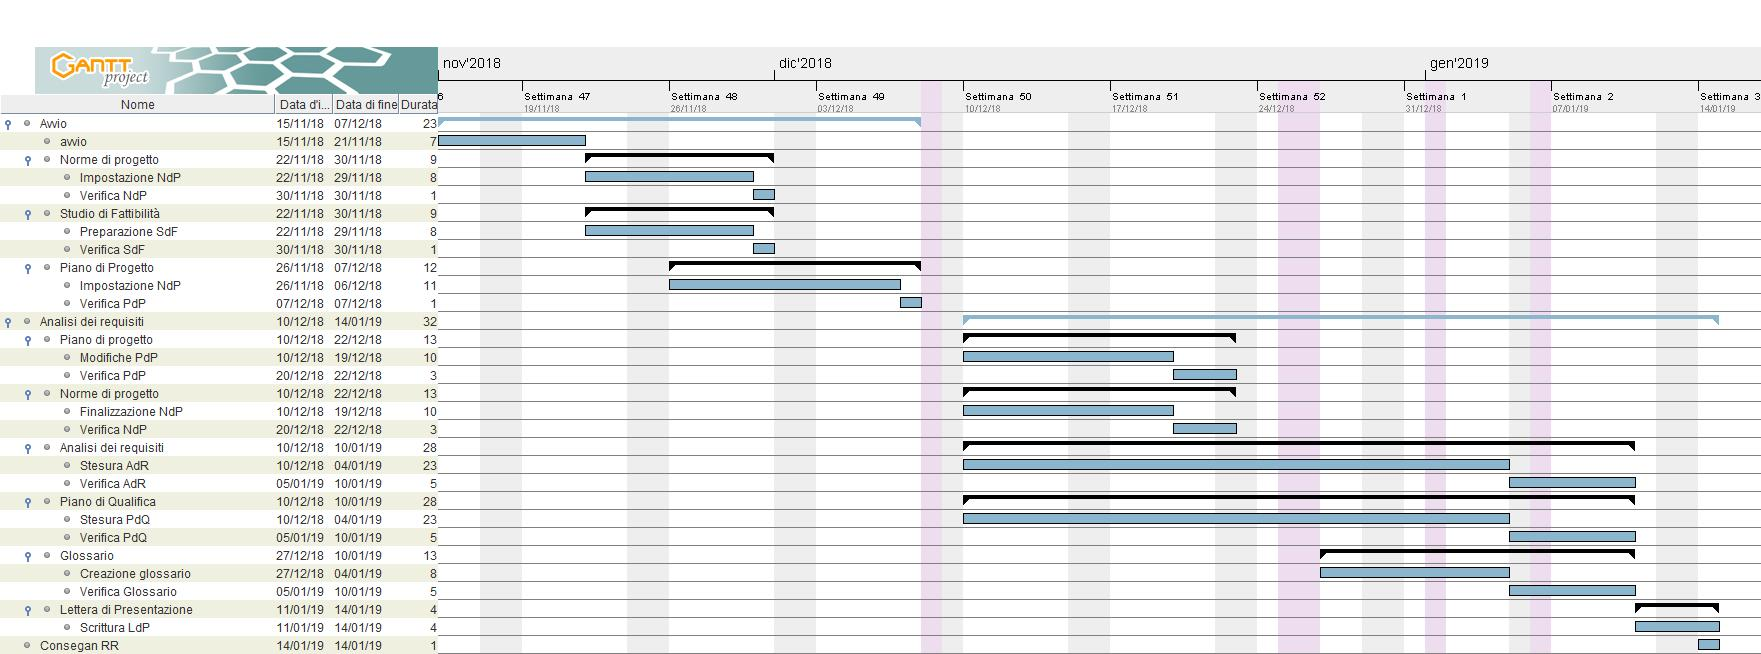
\includegraphics[width=\textwidth]{Gantt_terza_fase.jpg}
	\caption{Diagramma di Gantt del periodo di Progettazione di dettaglio e codifica}
\end{figure}

\begin{figure}[!htpb]
	\centering
	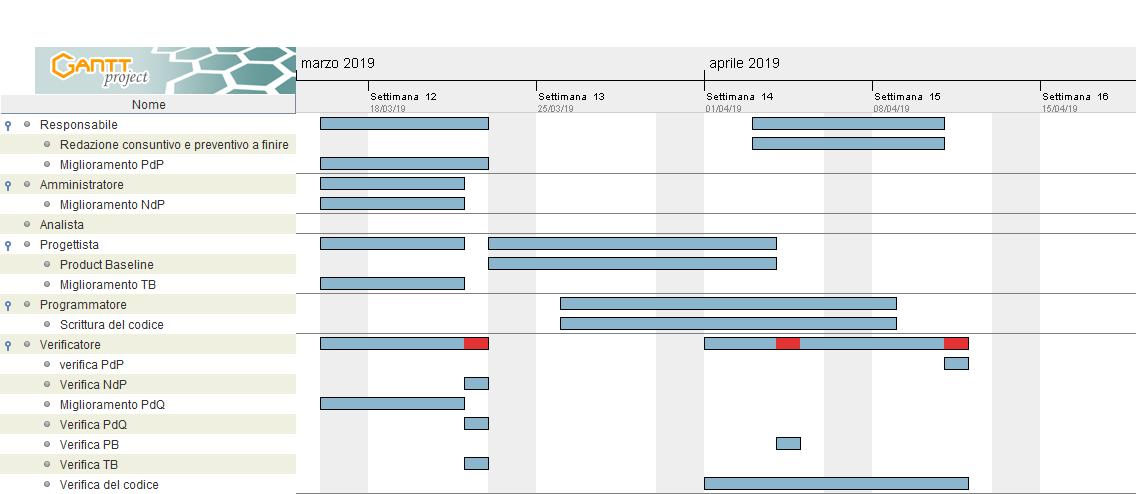
\includegraphics[width=\textwidth]{Gantt_terza_fase_risorse.jpg}
	\caption{Diagramma di Gantt delle risorse del periodo di Progettazione di dettaglio e codifica}
\end{figure}

\begin{table}[!htpb]
	\centering
	\renewcommand{\arraystretch}{2} 
	\rowcolors{2}{gray!25}{white}
	\begin{tabular}{|l|p{5cm}|p{5cm}|}
		\rowcolor{orange!50}
		\multicolumn{3}{|c|}{\textbf{Suddivisione temporale}}\\
		\hline
		\textbf{Ruolo} & \textbf{16/03/19 - 29/03/19} & \textbf{29/03/19 - 12/04/19} \\
		\hline
		\textbf{Responsabile} & \mat & \mar \\
		\hline
		\textbf{Amministratore} & \gia & \daG  \\
		\hline
		\textbf{Analista} & - & -  \\
		\hline
		\textbf{Progettista} & \parbox{5cm}{\pie \\ \mic} & \daL \\
		\hline
		\textbf{Programmatore} & \parbox{5cm}{\daG \\ \mar}& \parbox{5cm}{\mat \\ \mic \\ \pie}\\
		\hline
		\textbf{Verificatore} & \daL & \gia \\
		\hline
	\end{tabular}
	\caption{Suddivisione temporale del periodo di Progettazione di dettaglio e codifica}
\end{table}

\clearpage
\subsection{Validazione e collaudo}
	\subsubsection{Prospetto orario}
	La distribuzione oraria della fase di Validazione e collaudo è la seguente:
	
	\begin{table}[!htpb]
		\centering
		\renewcommand{\arraystretch}{2} 
		\rowcolors{2}{gray!25}{white}
		\begin{tabular}{|l c c c c c c|c| }
			\rowcolor{orange!50}
			\hline
			\multicolumn{8}{|c|}{\textbf{Suddivisione delle ore nei vari ruoli}}\\
			\hline
			\textbf{Nominativo} & RES 	& AMM 	& ANA 	& PRO 	& PRG 	& VER 	& \textbf{Totale} \\
			\hline
			\mat  				&-		& 12	&-		&-		&-		& 9		&21 \\
			\hline
			\pie  				&-		& 12	&-		&-		&-		& 9		&21\\
			\hline
			\mic  				&-		&-		&-		&-		& 6		& 15	&21\\
			\hline
			\mar  				&-		&-		&-		&-		& 10	& 11	&21\\
			\hline
			\daG  				& 8		&-		&-		&-		&-		& 13	&21\\
			\hline
			\daL  				&-		&-		&-		&-		&-		& 21	&21\\
			\hline
			\gia  				& 8		&-		&-		&-		&-		& 13	&21\\
			\hline
		\end{tabular}
		\caption{Suddivisione ore del periodo di Validazione e collaudo}
	\end{table}
	~\newline
	Di seguito rappresentata anche in un grafico:
\begin{figure}[!htpb]
	\centering
	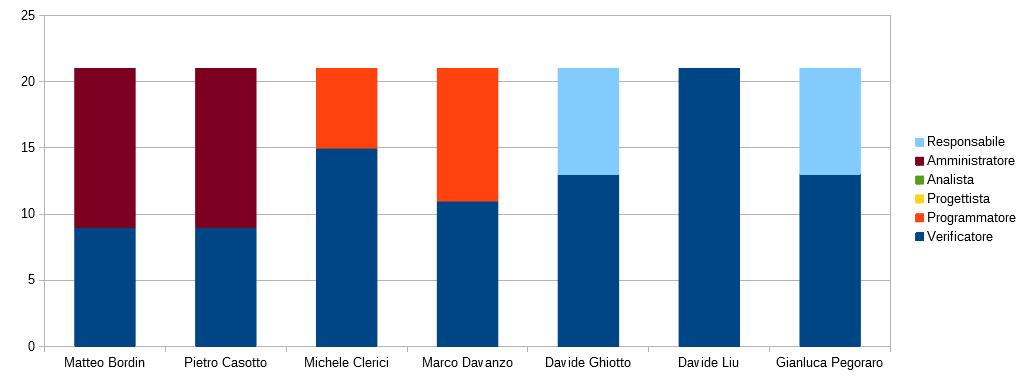
\includegraphics[width=\textwidth]{preventivo/grafico_quarta_parte.jpg}
	\caption{Grafico suddivisione oraria nel periodo di Validazione e collaudo}
\end{figure}
	\newpage
	\subsubsection{Conteggio ore}
	La distribuzione delle ore nei vari ruoli nella fase di Validazione e collaudo è la seguente:
	
	\begin{table}[!htpb]
			\centering
		\renewcommand{\arraystretch}{1.8} 
		\rowcolors{2}{gray!25}{white}
		\begin{tabular}{| c c c|}
			\rowcolor{orange!50}
			\hline
			\multicolumn{3}{|c|}{\textbf{Suddivisione delle ore nei vari ruoli}}\\
			\hline
			\textbf{Ruolo} 			& Ore 	& Costo\\
			\hline
			\textbf{Responsabile}	&16		&480\\
			\hline
			\textbf{Amministratore}	&24		&480\\
			\hline
			\textbf{Analista}		&0		&0\\
			\hline
			\textbf{Progettista}	&0		&0\\
			\hline
			\textbf{Programmatore}	&16		&240\\
			\hline
			\textbf{Verificatore} 	&91		&1365\\
			\hline
			\textbf{Totale} 		&147	&2565\\
			\hline 
		\end{tabular}
		\caption{Ore e costi totali del periodo di Validazione e collaudo}
	\end{table}
	~\newline Di seguito rappresentata anche in un grafico:
\begin{figure}[!htpb]
	\centering
	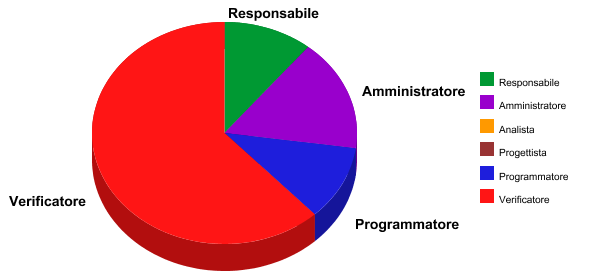
\includegraphics[scale=0.8]{preventivo/torta_quarta_parte.png}
	\caption{Grafico suddivisione ruoli nel periodo di Validazione e collaudos}
\end{figure}
\clearpage

\clearpage
